\chapter{초공간과 초대칭 동역학의 구성}

\lectureoverview{초대칭이 작용할 수 있는 가장 작은 계, 즉 에너지가 같은 보손 조화진동자 하나와 페르미온 조화진동자 하나에서 출발해 초대칭을 다시 구성한다. 두 계의 방정식이 각각 2계와 1계라는 차이에서 초전하와 그 대수가 나온다. 이어서 그 대수를 보통 좌표 (t)와 그라스만 좌표 \(\theta,\bar\theta\)를 갖는 공간 위의 기하학으로 재해석한다. 초장은 보손, 페르미온, 보조장을 하나의 대상으로 묶고, 베레진 적분은 불변인 보통 라그랑지안을 추출하며, 공변미분은 대칭과 양립하는 제약을 가능하게 한다. 카이랄 제약은 그 첫 번째 중요한 예다. 이 강의에서는 이 형식론에서 부호와 순서를 다루기 어렵다는 점을 숨기지 않고 보여준 뒤, 대칭 자체가 파인만 규칙의 목록보다 왜 더 근본적인지 설명하며 마무리한다.}

\section{한 모드 계로 돌아가기}

정지한 페르미온과 보손에서 다시 시작하자. 모든 공간 좌표와 운동량 표기는 생략한다. 각 모드에는 양자가 있거나 없으며, 생성 연산자와 소멸 연산자만으로 이를 기술할 수 있다. 보손 모드는 \(a^\dagger,a\), 페르미온 모드는 \(c^\dagger,c\)로 쓰자. 이들은 다음 관계를 만족한다.
\begin{align}
[a,a^\dagger]&=1,
&
\{c,c^\dagger\}&=1,
&
c^2=(c^\dagger)^2&=0.
\end{align}
두 양자의 에너지가 같아 \(m\)이면, 무시해도 되는 진공 상수를 제외하고 해밀토니안은 다음과 같다.
\begin{equation}
H=m\left(a^\dagger a+c^\dagger c\right).
\label{eq:l7-one-mode-hamiltonian}
\end{equation}
수 연산자 \(a^\dagger a\)는 음이 아닌 정수 값을 취할 수 있지만, \(c^\dagger c\)은 0 또는 1만 취할 수 있다. 이것이 이 장난감 모형의 운동학 전부다.

이 단순화는 전략적인 선택이다. 에너지를 바꾸지 않으면서 보손을 없애고 페르미온을 넣거나, 그 반대의 일을 하는 연산을 이해하고자 한다. 하지만 그 연산을 구성하기 전에, 같은 계를 연산자 언어에서 라그랑지안 언어로 옮겨 보자.

\section{보손 조화진동자}

보손에 대해 실수 좌표 \(\phi(t)\)를 도입하자. 공간적으로 변하지 않는 자유 스칼라장은 보통 조화진동자가 된다. 칠판에 처음 적힌 식은 다음과 같았다.
\[
\frac{1}{2}\dot\phi^{,2}+\frac{1}{2}m^2\phi^2.
\]
이 식은 운동에너지와 퍼텐셜에너지의 합이지 라그랑지안이 아니다. 강의에서는 곧바로 부호를 바로잡는다.
\begin{equation}
L_B=\frac{1}{2}\dot\phi^{,2}-\frac{1}{2}m^2\phi^2.
\label{eq:l7-boson-lagrangian}
\end{equation}

\begin{figure}[H]
\centering
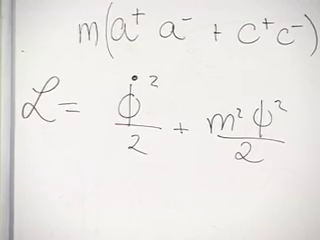
\includegraphics[width=0.62\textwidth]{lecture_07_figure_02.png}
\lectureframe{00:03:25.431}
\caption{보손 라그랑지안 위에 놓인 한 모드 해밀토니안. 화면은 말로 수정하기 전의 처음 부호가 플러스였던 점을 보존한다. \(T-V\)}
\end{figure}

\begin{classroomqa}
\audiencequestion{화면에 표시된 조화진동자 라그랑지안에서 부호가 잘못된 이유는 무엇인가? \lecturetimestamp{00:04:00}}
\lecturerresponse{에너지는 \(T+V\)이지만 라그랑지안은 \(T-V\)이다. 따라서 퍼텐셜 항에는 마이너스 부호가 붙어야 한다. 이 수정으로 방정식은 지수적으로 변하는 거동을 나타내는 식에서 의도한 조화진동을 나타내는 식으로 바뀐다.}
\end{classroomqa}

실제로 오일러--라그랑주 방정식은 다음을 준다.
\begin{align}
\frac{d}{dt}\frac{\partial L_B}{\partial\dot\phi}
&=\frac{\partial L_B}{\partial\phi},\\
\ddot\phi&=-m^2\phi,
\end{align}
즉,
\begin{equation}
\ddot\phi+m^2\phi=0.
\label{eq:l7-boson-eom}
\end{equation}
진동수는 \(m\)이지 \(m^2\)가 아니다. 이 조화진동자를 양자화하면 식 ~\eqref{eq:l7-one-mode-hamiltonian}의 \(a^\dagger\)와 \(a\)가 기술하는 것과 같은 상태 사다리를 얻는다.

\section{페르미온 작용이 1계인 이유}

페르미온 라그랑지안은 시간 미분이 하나뿐이어서 더 단순해 보인다. 그 이유는 의도적으로 단순한 시도에서 이미 드러난다. 서로 교환하는 보통 변수에 대해서는
\begin{equation}
L_{\mathrm{trial}}=\phi\dot\phi
=\frac{1}{2}\frac{d}{dt}\phi^2.
\end{equation}
이것은 전미분이다. 이에 따른 오일러--라그랑주 방정식은 \(\dot\phi=\dot\phi\)만을 말하므로, 미분 가능한 모든 경로가 허용된다. 작용에서 전미분을 빼도 끝점 자료는 달라지지만 운동 방정식의 벌크 부분은 달라지지 않는다.

이제 변수를 \(\psi\)로 바꾸고 그라스만 홀수 변수라고 하자. \(\psi\)와 \(\dot\psi\)는 모두 반교환한다. 왼쪽 변분을 택하면 홀수 인자들의 순서를 바꿀 때 마이너스 부호가 생기므로, 같은 형식의 시도에서 다음을 얻는다.
\begin{equation}
\frac{d}{dt}\frac{\partial L_{\mathrm{trial}}}{\partial\dot\psi}
=\dot\psi,
\qquad
\frac{\partial L_{\mathrm{trial}}}{\partial\psi}
=-\dot\psi.
\end{equation}
따라서 방정식은 다음과 같다.
\begin{equation}
\dot\psi=-\dot\psi
\quad\Longrightarrow\quad
\dot\psi=0.
\label{eq:l7-constant-fermion}
\end{equation}
서로 교환하는 좌표에서는 항등식에 불과했던 식이 반교환하는 좌표에서는 동역학적 내용을 갖게 되었다. 이 식은 조화진동자를 기술하기에는 내용이 지나치게 많아서 상수해만 허용하지만, 바로 그것이 필요한 실마리다.

\begin{classroomqa}
\audiencequestion{해가 단지 \(\psi\)가 상수라는 뜻인가? \lecturetimestamp{00:13:57}}
\lecturerresponse{그렇다. 식~\eqref{eq:l7-constant-fermion}은 실제 1계 미분방정식이며, 그 해는 임의의 그라스만 값 상수다. 질량항을 더하면 이 정적인 해가 진동하는 해로 바뀐다.}
\end{classroomqa}

당연해 보이는 시도인 \(m\psi^2\)는 \(\psi^2=0\)이므로 실패한다. 실수 홀수 변수 \(\psi_1,\psi_2\) 두 개가 필요하며, 이는 복소 변수 하나와 그 켤레로 바꾸어 쓸 수 있다. 강의에서는 칠판에 실수 변수 두 개를 쓰는 형식을 전개하며 부호와 2의 인자를 거듭 확인한다. 표준적인 정규화를 택한 복소 형식은 다음과 같다.
\begin{equation}
L_F=\frac{i}{2}
\left(\bar\psi\dot\psi-\dot{\bar\psi}\psi\right)
-m\bar\psi\psi.
\label{eq:l7-fermion-lagrangian}
\end{equation}
전미분을 무시하면 이는 \(i\bar\psi\dot\psi-m\bar\psi\psi\)이다. \(\bar\psi\)에 대해 변분하면 다음을 얻는다.
\begin{equation}
i\dot\psi=m\psi,
\qquad
\psi(t)=\psi(0)e^{-imt}.
\label{eq:l7-fermion-eom}
\end{equation}
켤레 방정식은 위상 부호가 반대다. 따라서 페르미온 모드는 보손 모드와 마찬가지로 에너지 \(m\)로 진동하지만, 그 방정식은 2계가 아니라 1계다.

\editorialnote{방정식~\eqref{eq:l7-fermion-lagrangian}은 실수 변수 두 개를 사용하는 탐색적 계산에서 표준적인 배열과 정규화 한 가지를 정한다. 강의에서는 여기에 \(i\)를 곱하고, 계수를 두 배 조정하며, 실수 성분 하나의 부호는 확정하지 않는다. 이러한 차이에도 핵심 결론은 달라지지 않는다. 페르미온의 운동항은 일차 미분형이고, 질량은 선형으로 나타나며, 복소 페르미온은 영이 아닌 쌍선형항을 만든다.}

이는 익숙한 상대론적 대비를 0차원으로 축소한 모습이다. 클라인--고든 방정식은 시간에 대해 2계인 반면, 디랙 방정식은 1계다. 공간을 생략하면 보손은 조화진동자 하나가 되고 페르미온은 복소 그라스만 조화진동자 하나가 된다.

\begin{classroomqa}
\audiencequestion{\(\psi\)와 \(\dot\psi\) 및 그 켤레를 쓰는 순서가 중요한가? \lecturetimestamp{00:18:58}}
\lecturerresponse{홀수 인자가 반교환하므로 중간 식은 순서에 따라 달라진다. 하지만 왼쪽 변분 또는 오른쪽 변분, 켤레화, 적분에 이르기까지 하나의 규약을 일관되게 사용하면 물리 이론은 임의의 표기 선호에 좌우되지 않는다. 홀수 인자 한 쌍의 순서를 뒤집으면 부호가 바뀌며, 다른 모든 곳에서도 일관되게 부호를 바꾸어야 한다.}
\end{classroomqa}

식~\eqref{eq:l7-boson-lagrangian}과 \eqref{eq:l7-fermion-lagrangian}를 결합하면 식~\eqref{eq:l7-one-mode-hamiltonian}이 나타내는 동일한 에너지 짝을 라그랑지안으로 기술할 수 있다. 이제 두 모드 사이의 대칭을 확인할 준비가 되었다.

\section{초전하와 그 대수}

페르미온을 없애고 보손을 넣는 연산자는 다음과 같다.
\begin{equation}
Q^\dagger=\sqrt{2m}\,a^\dagger c,
\end{equation}
켤레 연산자는 보손을 없애고 페르미온을 넣는다.
\begin{equation}
Q=\sqrt{2m}\,a c^\dagger.
\end{equation}
대수의 표준형을 얻도록 정규화를 택했다. \(cc^\dagger=1-c^\dagger c\), \(aa^\dagger=a^\dagger a+1\)와 보손 연산자와 페르미온 연산자가 서로 교환한다는 사실을 사용하면,
\begin{align}
\{Q,Q^\dagger\}
&=2m\left(ac^\dagger a^\dagger c+a^\dagger c a c^\dagger\right)\notag\\
&=2m\left[(a^\dagger a+1)c^\dagger c
+a^\dagger a(1-c^\dagger c)\right]\notag\\
&=2m\left(a^\dagger a+c^\dagger c\right)=2H.
\label{eq:l7-superalgebra}
\end{align}
보손 연산자는 페르미온 연산자를 지나 이동할 수 있다. 페르미온 점유를 제한하는 같은 멱등성으로부터 다음을 얻는다.
\begin{equation}
Q^2=(Q^\dagger)^2=0.
\end{equation}
마지막으로,
\begin{equation}
[H,Q]=[H,Q^\dagger]=0.
\label{eq:l7-conserved-supercharges}
\end{equation}
각 초전하는 보손 수와 페르미온 수를 서로 반대 방향으로 바꾼다. 따라서 진동수가 같으면 두 변화에 따른 에너지가 상쇄된다.

\begin{classroomqa}
\audiencequestion{\([H,Q]\)는 무엇인가? 답은 \(Q\)에 비례하는가? \lecturetimestamp{00:25:10}}
\lecturerresponse{아니다. 답은 0이다. 생성 또는 소멸 연산자 하나만 있다면 \(H\)와의 교환에서 그 에너지가 드러나겠지만, \(Q\)에 들어 있는 보손 항과 페르미온 항은 서로 상쇄된다. 이 상쇄가 바로 두 에너지가 같다는 조건이다.}
\end{classroomqa}

\begin{classroomqa}
\audiencequestion{그 교환자를 칠판에 이미 쓰지 않았나? \lecturetimestamp{00:25:45}}
\lecturerresponse{그렇다. 다시 찾아내는 과정은 관계를 그저 베끼지 않고 해석하게 해 준다는 점에서 유용하다. 해밀토니안과 교환한다는 것은 그 변환이 대칭이며 그 생성자가 보존된다는 뜻이다.}
\end{classroomqa}

\emph{전하}라는 말은 이 보존 법칙을 가리킨다. 그렇다고 \(Q\)을 상태에 붙는, 동시에 측정할 수 있는 보통 수처럼 취급해서는 안 된다. 이것은 그라스만 홀수이고 멱영이며 보손 상태를 페르미온 상태로 사상한다. 유용한 진술은 이것이 축퇴 초다중항 안에서 작용하는 보존 생성자라는 것이다.
\editorialnote{이 설명은 상태를 에너지나 전하로 분류하는 교실의 비유를 더 정확하게 다듬는다. 개별적인 비에르미트 홀수 초전하는 수치 양자값을 갖는 보통 관측량이 아니다. 올바른 분류는 이들의 보존된 작용과 완전한 초대수의 표현으로 주어진다.}

\section{미분 연산자로서의 생성자}

대수는 간결하지만, 그것만으로는 상호작용 이론을 어떻게 구성할지 알 수 없다. 다음 단계는 기하학이다. 익숙한 대칭 생성자도 이미 미분 연산자로 작용한다. 강의의 규약에서는
\begin{equation}
H=i\frac{\partial}{\partial t},
\qquad
P=-i\frac{\partial}{\partial x}.
\end{equation}

\begin{figure}[H]
\centering
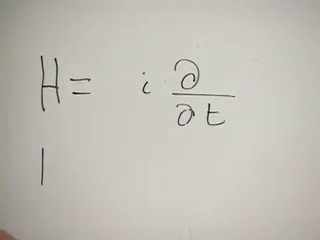
\includegraphics[width=0.50\textwidth]{lecture_07_figure_03.png}
\lectureframe{00:28:12.720}
\caption{시간 병진의 생성자로 나타낸 해밀토니안.}
\end{figure}

각운동량도 마찬가지로 좌표와 미분의 곱이다. 초전하가 홀수 생성자라면 홀수 좌표에 대한 미분으로 나타낼 수 있는지 묻는 것이 자연스럽다. 따라서 시간축을 다음 초공간으로 확장한다.
\begin{equation}
(t,\theta,\bar\theta),
\qquad
\theta^2=\bar\theta^2=0,
\qquad
\theta\bar\theta=-\bar\theta\theta.
\end{equation}
이 공간 위의 장은 보통 시간과 켤레인 그라스만 좌표 한 쌍에 의존한다.

강의에서는 부호가 얼마나 까다로운지 의도적으로 드러낸다. 복소켤레를 취할 때 생기는 부호, 홀수 매개변수를 옮길 때 생기는 부호, 왼쪽 미분과 오른쪽 미분 중 어느 쪽을 택하느냐에 따른 부호는 서로 다른 연산에서 나온다. 서로 양립하지 않는 칠판상의 전개 단계를 그대로 유지하는 대신, 여기서는 하나의 규약을 정한다. 모든 홀수 미분은 왼쪽 미분으로 둔다.
\begin{equation}
q=\partial_\theta+i\bar\theta\partial_t,
\qquad
\bar q=\partial_{\bar\theta}+i\theta\partial_t.
\label{eq:l7-differential-supercharges}
\end{equation}
그러면
\begin{equation}
q^2=\bar q^{,2}=0,
\qquad
\{q,\bar q\}=2i\partial_t=2H.
\label{eq:l7-differential-algebra}
\end{equation}
두 배 인자는 두 교차항 \(\{\partial_\theta,\theta\}=1\)와 \(\{\partial_{\bar\theta},\bar\theta\}=1\)에서 나온다. 생성자에 \(\partial_\theta\)와 \(\partial_{\bar\theta}\)만 들어 있다면 반교환자는 영이 되어 해밀토니안을 재현할 수 없다.

\begin{classroomqa}
\audiencequestion{\(q\)와 \(\bar q\)의 시간 미분 항 두 개는 같은 부호를 가져야 하나? \lecturetimestamp{00:31:01}}
\lecturerresponse{혼합 반교환자가 \(2H\)이 되도록 부호를 일관되게 정해야 한다. 전체적으로 플러스인 규약이나 그에 맞게 켤레를 취한 규약을 모두 사용할 수 있다. 기호 \(i\)에 대한 직관이 아니라 계산이 상대 부호를 정한다.}
\end{classroomqa}

강의실에서는 부호를 거듭 확인하고, 출근길에 부호가 바뀌는 것 같다는 농담도 나온다. 적절한 농담이다. 물리적 규약이 전혀 바뀌지 않았더라도 그라스만 매개변수를 좌표 사이로 옮기면 부호가 바뀔 수 있다. 뒤에 나오는 모든 내용은 식~\eqref{eq:l7-differential-supercharges}을 고정된 기준으로 삼는다.

\subsection{좌표 이동으로서의 초대칭}

무한소 홀수 매개변수 \(\xi,\bar\xi\)를 두자. 초장에
\begin{equation}
\delta_\xi=\xi q+\bar\xi\bar q
\end{equation}
를 작용시키는 것은 위 규약에서 다음 무한소 좌표 변환과 동등하다.
\begin{align}
\theta&\longrightarrow\theta+\xi,\\
\bar\theta&\longrightarrow\bar\theta+\bar\xi,\\
t&\longrightarrow t+i\left(\xi\bar\theta+\bar\xi\theta\right).
\label{eq:l7-coordinate-shift}
\end{align}
따라서 스칼라 초장의 변화는 다음과 같다.
\begin{equation}
\delta_\xi\Phi
=\left(\xi\partial_\theta+\bar\xi\partial_{\bar\theta}
+i\xi\bar\theta\partial_t+i\bar\xi\theta\partial_t\right)\Phi
=\left(\xi q+\bar\xi\bar q\right)\Phi.
\end{equation}
이것이 초대칭의 기하학적 내용이다. 이는 홀수 방향으로의 병진이며, 보통 시간 방향의 병진과 결부되어 있다. 홀수 이동 두 번의 합성은 식~\eqref{eq:l7-differential-algebra}에 따라 시간 병진으로 닫힌다.

\begin{classroomqa}
\audiencequestion{논란이 된 마이너스 부호는 시간을 거슬러 움직인다는 뜻일 수 있나? \lecturetimestamp{00:58:13}}
\lecturerresponse{다른 부호 규약을 택하면 표시된 무한소 시간 이동의 방향이 반대가 될 수 있지만, 별개의 물리적 과거 방향 시간 과정이 도입되는 것은 아니다. 중요한 것은 좌표 변환과 미분 생성자가 같은 대수를 따른다는 점이다.}
\end{classroomqa}

\begin{classroomqa}
\audiencequestion{이렇게 확장한 시간에는 물리적 실현이 있는가, 아니면 형식적인 계산 도구일 뿐인가? \lecturetimestamp{00:58:23}}
\lecturerresponse{유용한 의미에서 이는 대수를 기하학으로 묶어 표현하는 계산 도구다. 하지만 상호작용을 도입하면 그 표현이 물리적으로 유용해진다. 초공간은 텐서 미적분이 로런츠 스칼라를 구성하는 데 도움이 되듯, 모든 단계에서 보손--페르미온 대칭을 보존하는 라그랑지안을 구성하는 체계적인 계산법을 제공한다.}
\end{classroomqa}

\section{초장과 보조 성분}

홀수 좌표가 둘뿐이므로 짝수 초장의 전개는 유한한 항에서 끝난다.
\begin{equation}
\Phi(t,\theta,\bar\theta)
=\phi(t)+\bar\theta\psi(t)+\bar\psi(t)\theta
+D(t)\bar\theta\theta.
\label{eq:l7-superfield}
\end{equation}
짝수 차수 단항식 \(\phi\)와 \(D\)의 계수는 보손이고, 홀수 차수 단항식 \(\psi\)와 \(\bar\psi\)의 계수는 페르미온이다. \(\theta^2\), \(\bar\theta^2\) 또는 그 이상의 항은 남지 않는다. \(t\)에 대한 보통 테일러 급수는 유한한 항에서 끝나지 않고 여기서는 쓸모가 없으므로 시간 의존성은 전개하지 않는다.

\begin{classroomqa}
\audiencequestion{맨 위 항의 성분 \(D(t)\)는 무엇인가? \lecturetimestamp{00:41:46}}
\lecturerresponse{이 단계에서는 유한 전개에서 마지막에 놓인 보손 계수일 뿐이다. 성분 작용에서는 보통 운동항이 없고 대수적인 운동 방정식으로 제거되므로 보조장이라고 부른다. 강의에서는 ``D는 dummy의 D''라는 장난스러운 설명도 나오는데, 이는 이 장의 비동역학적 역할을 잘 나타내지만 역사적 정의는 아니다.}
\end{classroomqa}

초장은 하나의 대상이고 \(\phi,\psi,\bar\psi,D\)는 그 성분들이다. 초대칭 변환은 이 성분들을 서로 섞는다. 따라서 보손과 페르미온은 벡터의 \(x\) 성분과 \(y\) 성분이 회전으로 서로 연결되는 것과 구조적으로 매우 비슷한 방식으로 관련되어 있다. 다만 그라스만 방향을 보통 축처럼 그릴 수는 없다.

\section{초작용과 맨 위 성분}

운동 방정식을 얻으려면 작용이 필요하다. 보통 장론에서는 스칼라 라그랑지안을 만든 뒤 시공간에 대해 적분한다. 여기서 이에 대응하는 식은 다음과 같다.
\begin{equation}
S=\int dt\,d\theta\,d\bar\theta\;\Lambda
\bigl(\Phi,\text{ superspace derivatives of }\Phi\bigr),
\label{eq:l7-superaction}
\end{equation}
여기서 \(\Lambda\)은 짝수 초장이다. 베레진 적분은 대수적이다. 다음을 택하자.
\begin{equation}
\int d\theta\,d\bar\theta\;\bar\theta\theta=1.
\end{equation}
따라서
\begin{equation}
\Lambda=A+\bar\theta B+\bar B\theta+C\bar\theta\theta,
\end{equation}
이면,
\begin{equation}
\int d\theta\,d\bar\theta\;\Lambda=C.
\label{eq:l7-top-component}
\end{equation}
홀수 적분은 맨 위 성분을 추출해 남기며, 이를 시간에 대해 적분하면 보통 라그랑지안을 얻는다.

결과가 불변인 이유는 무엇일까? 초대칭 변환은 적분 변수를 평행이동시킨다. 최고 성분의 변분은 시간에 대한 통상적인 전미분인 반면, 홀수 전미분은 베레진 적분에서 사라진다. 적절한 경계 조건 아래에서 작용은 변하지 않는다. 이는 시공간에 대해 적분하기 전에 로런츠 스칼라를 구성하는 것에 대응하는 초공간의 방법이다.

\section{초장 곱하기}

기존 초장으로 새 초장을 만드는 가장 간단한 방법은 그 초장을 자기 자신과 곱하는 것이다. 식~\eqref{eq:l7-superfield}에서 시작하면 \(\theta^2\) 또는 \(\bar\theta^2\)가 포함된 모든 항은 사라진다. 순서를 \(\bar\theta\theta\)로 유지하고 켤레 성분장을 왼쪽에 쓰면 다음을 얻는다.
\begin{align}
\Phi^2
={}&\phi^2
+2\phi\bar\theta\psi
+2\phi\bar\psi\theta\notag\\
&+\left(2\phi D-2\bar\psi\psi\right)\bar\theta\theta.
\label{eq:l7-superfield-square}
\end{align}

\begin{figure}[H]
\centering
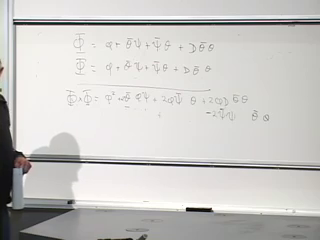
\includegraphics[width=0.82\textwidth]{lecture_07_figure_05.png}
\lectureframe{01:07:57.844}
\caption{성분별로 전개한 초장 곱과 그 \(\bar\theta\theta\) 항들을 모아 나타낸 그림.}
\end{figure}

두 항 \(\phi D\)와 \(D\phi\)는 둘 다 짝수장이므로 더해진다. 두 페르미온 교차항도 각각 순서를 바꾸면 더해지지만, 두 항 모두 마이너스 부호를 갖는다.
\begin{equation}
(\bar\theta\psi)(\bar\psi\theta)
+(\bar\psi\theta)(\bar\theta\psi)
=-2\bar\psi\psi\,\bar\theta\theta.
\end{equation}
제곱을 홀수 좌표에 대해 적분하면 다음을 얻는다.
\begin{equation}
\int d\theta\,d\bar\theta\;\Phi^2
=2\phi D-2\bar\psi\psi.
\end{equation}
이 항은 구성상 초대칭이지만, 아직 운동항을 갖는 라그랑지안은 아니다. 시간 미분이 없다.

이어서 칠판에는 \(\Phi^3\), \(\Phi^4\), \(\Phi^n\)를 연습 문제로 제시한다. 간단한 규칙이 있다. 임의의 보통 함수 \(W\)에 대해
\begin{equation}
\left.W(\Phi)\right|_{\bar\theta\theta}
=W'(\phi)D-W''(\phi)\bar\psi\psi.
\label{eq:l7-function-top-component}
\end{equation}
\(W(\phi)=\phi^2\)의 경우에는 식~\eqref{eq:l7-superfield-square}가 재현되고, \(W(\phi)=\phi^n\)의 경우에는 다음을 얻는다.
\begin{equation}
\left.\Phi^n\right|_{\bar\theta\theta}
=n\phi^{n-1}D-n(n-1)\phi^{n-2}\bar\psi\psi.
\end{equation}
\editorialnote{\(n\)제곱의 경우는 연습 문제로 제시하면서 예상되는 항의 종류를 설명한다. 식~\eqref{eq:l7-function-top-component}은 고정된 순서 규약에서 완성된 규칙을 제공한다.}

이때 강사는 강의실 사람들이 지쳤는지 묻는다. 청중은 아니라고 답하고, 강사는 자신은 지쳤다고 말한다. 이 대화는 단순한 웃음거리에 그치지 않는다. 초장 거듭제곱은 전개가 유한하게 끝나므로 다루기 쉽지만, 부호 계산이 실제로 까다로워지는 곳은 미분과 제약이다.

\section{초대칭을 따르는 미분은 무엇인가?}

다음 칠판 논의를 따라가기 전에 한 가지를 바로잡아야 한다. 보통 시간 미분은 문제가 없다.
\begin{equation}
[\partial_t,q]=[\partial_t,\bar q]=0.
\end{equation}
따라서 \(\Phi\)가 초장이면 \(\partial_t\Phi\)도 초장으로 변환된다. 까다로운 것은 맨몸 홀수 미분 \(\partial_\theta\Phi\)와 \(\partial_{\bar\theta}\Phi\)이다. 이 미분들은 두 초전하 모두와 반교환하지 않기 때문이다. 제약을 두고 초대칭 성분 구성을 명시적으로 하는 데에는 수정된 홀수 미분이 필요하다.
\editorialnote{시간 미분을 하면 또 다른 초장이 되지 않는다는 강의 중 발언은 여기서 사용한 규약에서는 옳지 않다. \(\partial_t\)는 두 초전하 모두와 교환하므로 공변적이다. 수정된 홀수 미분을 뒤이어 구성하는 과정은 여전히 필요하며, 그것이 강의에서 다루는 실제 수학적 요점이다.}

\subsection{``마법장 비유''}

강의에서는 보통 회전을 예로 들어 기준을 설명한다. \(f(x,y)\)가
\begin{equation}
\partial_y f=0.
\label{eq:l7-magic-constraint}
\end{equation}
을 만족한다고 하자. 이런 함수를 ``매직장''이라고 부르자. 이 함수는 \(x\)에는 의존하지만 \(y\)에는 의존하지 않는다. 회전해도 매직장들의 집합이 보존되는가? 다음에 대해서는
\begin{equation}
L_z=-i\left(x\partial_y-y\partial_x\right),
\end{equation}
다음이 성립한다.
\begin{equation}
[\partial_y,L_z]=i\partial_x\neq0.
\end{equation}
따라서 \(L_z f\)는 일반적으로 \(y\)에 의존하게 된다. 처음에 \(f\)가 식~\eqref{eq:l7-magic-constraint}을 만족하더라도 마찬가지다. 이 제약은 회전 불변이 아니다.

일반적인 원리는 간단하다. 장이 \(C\Phi=0\)을 만족하고 대칭이 \(G\)에 의해 생성된다면, \(C\)와 \(G\)의 등급 교환자가 영일 때 변환된 장도 제약 조건을 만족한다. 두 연산자가 모두 홀수이면 등급 교환자는 반교환자이다.

\begin{classroomqa}
\audiencequestion{장에 대한 제약이 대칭과 양립하는 조건은 무엇인가? \lecturetimestamp{01:17:56}}
\lecturerresponse{제약 연산자가 대칭 생성자들과 등급 교환할 때다. 그러면 \(C(G\Phi)\)에서 \(G\)를 옮겨 \(G(C\Phi)=0\)로 바꿀 수 있다. 회전 예에서는 \(\partial_y\)가 회전 생성자와 교환하지 않으므로 제약이 보존되지 않는다.}
\end{classroomqa}

\subsection{공변 홀수 미분}

초전하를 식~\eqref{eq:l7-differential-supercharges}로 정하고 다음을 정의하자.
\begin{equation}
\mathcal D=\partial_\theta-i\bar\theta\partial_t,
\qquad
\bar{\mathcal D}=\partial_{\bar\theta}-i\theta\partial_t.
\label{eq:l7-covariant-derivatives}
\end{equation}
바뀌는 것은 시간 미분 항의 부호뿐이다. 직접 계산하면 다음을 얻는다.
\begin{align}
\{\mathcal D,q\}
&=\{\mathcal D,\bar q\}
=\{\bar{\mathcal D},q\}
=\{\bar{\mathcal D},\bar q\}=0,\\
\{\mathcal D,\bar{\mathcal D}\}&=-2i\partial_t.
\label{eq:l7-covariant-algebra}
\end{align}
영이 아닐 수 있는 두 교차항은 서로 상쇄된다. 이는 홀수 연산자에 대응하는 공변미분이다. 변환 법칙을 보존하면서 미분한다.

강의에서는 보조 성분과 이 미분 연산자를 모두 \(D\)로 표기한다. 성분은 \(D(t)\)로 남겨 두고 연산자는 필기체 \(\mathcal D\)로 표기하겠다.

\section{카이랄 제약}

이제 초대칭 아래에서 보존되는 비자명한 제약을 부과할 수 있다.
\begin{equation}
\bar{\mathcal D}\Phi=0.
\label{eq:l7-chiral-constraint}
\end{equation}
이런 장을 카이랄이라고 한다. 초대칭 변환 전의 장이 카이랄이면,
\begin{equation}
\bar{\mathcal D}(q\Phi)
=-q(\bar{\mathcal D}\Phi)=0,
\qquad
\bar{\mathcal D}(\bar q\Phi)
=-\bar q(\bar{\mathcal D}\Phi)=0.
\end{equation}
따라서 변환된 초장 전체가 제약된 집합 안에 남는다. 매직장 조건과 달리 카이랄성은 대칭과 양립한다.

제약을 풀기 위해 이동된 시간 좌표를 정의하자.
\begin{equation}
\tau=t+i\bar\theta\theta.
\label{eq:l7-chiral-time}
\end{equation}
왼쪽 미분을 사용하므로
\begin{equation}
\partial_{\bar\theta}\tau=i\theta,
\end{equation}
따라서
\begin{equation}
\bar{\mathcal D}F(\tau,\theta)
=\left(\partial_{\bar\theta}-i\theta\partial_t\right)F(\tau,\theta)
=i\theta\partial_\tau F-i\theta\partial_\tau F=0.
\end{equation}
일반적인 국소 카이랄 초장은 \(\bar\theta\)에 \(\tau\)를 통해서만 의존한다.
\begin{equation}
\Phi_{\mathrm{ch}}(\tau,\theta)
=\phi(\tau)+\bar\psi(\tau)\theta.
\label{eq:l7-chiral-field-tau}
\end{equation}

\begin{classroomqa}
\audiencequestion{\(\tau\)와 \(\theta\)에 의존하는 형태만 카이랄 제약을 만족하는가? \lecturetimestamp{01:32:35}}
\lecturerresponse{국소적으로는 그렇다. 미분 방정식 \(\bar{\mathcal D}\Phi=0\)은 독립적인 \(\bar\theta\) 의존성을 이동된 좌표 \(\tau=t+i\bar\theta\theta\)에 흡수할 수 있다는 뜻이다. 나머지 유한 전개는 \(\tau\)의 함수와 \(\theta\)에 비례하는 항 하나로 이루어진다.}
\end{classroomqa}

원래 시간 좌표로 다시 전개하면,
\begin{align}
\phi(\tau)
&=\phi(t)+i\bar\theta\theta\dot\phi(t),\\
\bar\psi(\tau)\theta
&=\bar\psi(t)\theta,
\end{align}
두 번째 줄의 보정항은 \(\theta^2\)를 포함하기 때문이다. 따라서
\begin{equation}
\Phi_{\mathrm{ch}}(t,\theta,\bar\theta)
=\phi(t)+\bar\psi(t)\theta
+i\bar\theta\theta\dot\phi(t).
\label{eq:l7-chiral-field-components}
\end{equation}

\begin{classroomqa}
\audiencequestion{\(\phi(t+i\bar\theta\theta)\)의 테일러 전개에 2차 항도 들어가야 하지 않나? \lecturetimestamp{01:33:51}}
\lecturerresponse{아니다. 첫 번째 보정항은 \(i\bar\theta\theta\dot\phi\)이고, 그보다 높은 차수의 모든 보정항에는 \((\bar\theta\theta)^2=0\)가 들어간다. 청중은 이를 곧바로 알아차린다. 멱영성 때문에 이미 첫 두 항만 남고 급수가 끝난다.}
\end{classroomqa}

이것이 카이랄성의 간결함이다. 제약되지 않은 초장인 식~\eqref{eq:l7-superfield}에는 보손 성분 자리 두 개와 페르미온 성분 자리 두 개가 있다. 이 최소 1차원 예에서는 카이랄 조건이 독립적인 보조장 자리를 없애고 맨 위 성분을 \(\dot\phi\)에 결부한다.

\section{제대로 멈춘 계산}

자연스럽게 다음으로 할 일은 카이랄 장과 그 켤레를 결합해 초공간에서 적분하는 것이다. 켤레 전개를 시작하자 청중 한 사람이 켤레화할 때 순서 \(\theta\bar\theta\)를 뒤집어야 하는지 묻는다. 그 시점에는 부호를 더는 믿기 어렵다. 허세를 부리는 대신 계산을 멈춘다.

\begin{classroomqa}
\audiencequestion{켤레장 곱셈은 미루더라도 핵심 결과를 말해 줄 수 있는가? \lecturetimestamp{01:37:30}}
\lecturerresponse{그렇다. 부호와 켤레화를 일관되게 처리하면 카이랄 장과 그 켤레로 만든 초공간 식에서 원하는 보통 보손 및 페르미온 운동항을 얻는다. 이 강의의 중요한 결과는 믿기 어려운 계산 끝부분을 그대로 옮기는 것이 아니라 구성 원리다.}
\end{classroomqa}

계산을 멈춘 지점을 분명히 남겨 두어야 한다. 이 형식론에서는 홀수 인자 하나의 위치만 잘못되어도 부호가 바뀌며, 켤레화와 미분, 곱셈, 적분을 거치면서 같은 규약을 유지해야 한다. 그 연결이 끊겼다면 계속하기 전에 바로잡아야 한다. 표준 규약에서 익숙한 운동 작용은 켤레 곱으로 구성되지만, 성분으로 자세히 전개하는 일은 끝나지 않은 칠판 식을 복원하는 과정이 아니라 다음 번에 정확히 계산할 몫이다.

\section{대칭이 핵심인 이유}

초대칭 라그랑지안은 보손과 페르미온을 나란히 놓는 데 그치지 않는다. 이들의 질량과 상호작용을 제약해 초대수의 표현을 이루게 한다. 초대칭이 정확한 진공에서는 초다중항을 이루는 입자들의 질량이 같다. 이들의 고리 보정 기여는 서로 연관되어 있으며, 보손과 페르미온의 자외선 효과는 대칭이 정하는 조합에서 상쇄된다.

이 때문에 구성 형식론이 중요하다. 파인만 꼭짓점을 나열해 상쇄를 다이어그램마다 확인할 수도 있지만, 그러면 상쇄가 우연처럼 보인다. 초대칭은 로런츠 대칭이 모든 관성계에서 산란 진폭이 일관되게 변환되는 이유를 설명하는 것과 같은 방식으로 그 상쇄를 설명한다.

\editorialnote{정확한 초대칭이 개별 자체에너지 보정이 모두 사라진다는 뜻은 아니다. 초대칭은 재규격화를 서로 연관시키고 특정 자외선 민감성을 없애지만, 비재규격화 정리의 성립 여부는 대상량과 차원, 초대칭의 양에 달려 있다. 강의의 폭넓은 상쇄 주장은 이처럼 조건을 명시한 형태로 유지한다.}

\begin{classroomqa}
\audiencequestion{``카이랄''은 어떻게 철자하는가? \lecturetimestamp{01:39:48}}
\lecturerresponse{C-H-I-R-A-L. 이 말은 제약 \(\bar{\mathcal D}\Phi=0\)을 가리킨다. 3차원 공간에서 물체가 갖는 보통의 기하학적 손잡이성은 아니다. 다만 이 용어는 상대론적 스피너의 왼손 및 오른손 구조에서 유래했다.}
\end{classroomqa}

\begin{classroomqa}
\audiencequestion{라그랑지안을 거치지 않고 초대칭 파인만 규칙으로 바로 넘어갈 수 있는가? \lecturetimestamp{01:40:00}}
\lecturerresponse{규칙 자체를 제시할 수는 있지만, 결합상수 사이의 관계와 그에 따른 상쇄가 설명되지 않은 우연처럼 보일 것이다. 더 깊은 내용은 일반화된 시공간 대칭이다. 라그랑지안이나 그에 동등한 불변 형식은 그 이유를 드러내고 규칙을 체계적으로 도출한다.}
\end{classroomqa}

섭동의 모든 차수에서 로런츠 변환을 한 번도 언급하지 않았는데도 로런츠 불변 진폭이 나온다고 가정해 보자. 계산을 충분히 거듭하고 나면 우리는 설명을 요구할 것이다. 그 답은 모든 차수를 한꺼번에 조직하는 시공간 대칭일 것이다. 초공간의 역할도 이와 비슷하다. \(\theta,\bar\theta\)에서의 이동은 보손 성분과 페르미온 성분을 서로 섞으며, 그 대수는 시공간 병진으로 닫힌다.

\begin{classroomqa}
\audiencequestion{그라스만 좌표처럼 보통의 공간 좌표도 유한 거듭제곱 급수로 전개해야 하나요? \lecturetimestamp{01:44:55}}
\lecturerresponse{아니다. 보통 좌표에 대한 거듭제곱 급수는 끝나지 않으며, 대개 자연스러운 분해 방식도 아니다. 장을 파동과 운동량으로 분해하는 푸리에 변환이 더 유용하다. \(\theta\)로 전개하는 방식이 특별한 까닭은 멱영성 때문에 급수가 유한하게 끝나기 때문이다.}
\end{classroomqa}

\begin{classroomqa}
\audiencequestion{LHC에서 새로운 입자가 발견되면, 그것이 단지 미지의 입자가 아니라 초대칭 짝입자임을 어떻게 알아낼 수 있나요? \lecturetimestamp{01:45:42}}
\lecturerresponse{초대칭은 단지 하나의 추가 상태가 아니라 서로 연관된 양자수와 상호작용을 예측한다. 스핀은 1/2만큼 차이가 나고, 게이지 전하들은 서로 연관되며, 많은 세제곱 및 네제곱 결합은 일반적인 이론에서보다 적은 수의 독립 매개변수로 정해진다. 산란 단면적, 붕괴 분기비, 그리고 나머지 입자 스펙트럼이 이러한 관계들을 만족해야 한다.}
\end{classroomqa}

낯선 공명 하나만으로 초대칭이 입증되지는 않는다. 결합 상수와 입자 스펙트럼 사이의 관계망이 입증의 근거가 될 것이다. 이것이 초공간 구성에 대응하는 실험적 측면이다. 겉보기에는 서로 독립적인 성분 상호작용들이 하나의 불변량에서 나온다.

\begin{classroomqa}
\audiencequestion{관측된 입자와 가설적인 초대칭 짝입자의 질량은 같지 않습니다. 이것은 이론을 어떻게 바꾸나요? \lecturetimestamp{01:47:01}}
\lecturerresponse{이론을 크게 바꾼다. 초대칭은 깨져야 하며, 보통 자발적 대칭 깨짐이 관측 부문에 전달되는 방식으로 이루어진다. 대칭 깨짐은 다중항의 질량을 갈라놓으면서도 상호작용을 제어할 만큼, 그리고 깨짐 에너지 척도가 충분히 낮다면 자외선 보정을 제어할 만큼의 구조를 보존한다. 이 메커니즘을 구체적으로 밝히는 일은 그 자체로 상당한 이론적 과제이며, 중력을 포함하면 특히 그렇다.}
\end{classroomqa}

\section{단순한 원리, 어려운 계산}

마무리 평가는 유난히 솔직하다. 출발점의 발상은 단순해 보인다. 보손과 페르미온이 대칭으로 연결되어 있다는 것이다. 하지만 이를 구체화하는 과정은 곧 지표, 켤레, 그라스만 변수의 순서, 부호를 다루는 학문으로 발전한다. 대칭을 구성한 뒤에도 현실적인 입자물리학을 위해서는 대칭을 깨야 하며, 중력과 결합하면 초중력으로 이어져 구조가 한층 더 복잡해진다.

이 어려움이 발상이 공허하다는 증거는 아니다. 자연은 단순한 원리를 계산하기 쉽게 만들어야 할 의무가 없다. 전문가들은 부호 규칙이 몸에 밸 때까지 세부 계산을 거듭하며 이 주제를 익힌다. 답답함은 간결한 대수
\begin{equation}
\{Q,Q^\dagger\}=2H
\end{equation}
와 상호작용하는 이론에서 이를 구현하는 데 필요한 방대한 계산 체계 사이의 간극에서 생긴다.

\begin{classroomqa}
\audiencequestion{추상화의 층을 하나 더 쌓으면 결국 형식이 단순해지나요, 아니면 복잡성이 계속 늘어나나요? \lecturetimestamp{01:49:33}}
\lecturerresponse{세부 계산을 없애 주는 일반적인 단순화 방법은 없다. 기본 규칙은 짧을 수 있지만, 이를 믿을 수 있게 적용하려면 규약을 반복해서 정확히 다뤄야 한다. 그래서 이 주제를 제대로 다루려면 보통 광범위한 입자물리학 강의의 일부가 아니라 하나의 기술 과목 전체가 필요하다.}
\end{classroomqa}

\begin{classroomqa}
\audiencequestion{이 변환은 페르미온과 보손이 실제로 무엇인지, 또는 두 입자의 통상적인 거동이 왜 다른지를 알려 주나요? \lecturetimestamp{01:51:42}}
\lecturerresponse{두 입자가 하나의 초장(superfield)을 이루는 성분이며 초전하에 의해 서로 대응하는 상임을 알려 준다. \(Q\)을 작용시키면 보손 성분이 페르미온 성분으로 변환되고, 다음 변환에서는 미분과 보조 성분이 생긴다. 이는 회전이 벡터의 성분들을 서로 섞는 것과 비슷하지만, 똑같이 문자 그대로인 그림으로 옮길 수는 없다. 여기에 적합한 언어는 그라스만 기하학 자체다.}
\end{classroomqa}

이 답은 우리를 핵심 발상으로 되돌린다. 초대칭 변환은 초공간에서의 미소한 변환이다. 보통 회전이 성분들을 서로 섞듯이 \(\phi,\psi,\bar\psi,D\)를 서로 섞으며, 그 대수는 시간 병진으로 닫힌다. 이 그림은 추상적이지만 자의적이지 않다. 초장의 모든 항, 공변미분의 모든 부호, 성분 상호작용 사이의 모든 관계는 대수를 구현하기 위해 존재한다.

\section{우리가 구성한 것}

짝을 이루는 진동자 해밀토니안에서 시작해 서로 다른 두 가지 라그랑지안 기술을 되찾았다. 보손은 2계 진동자 방정식을 따르고, 페르미온에는 1계 그라스만 작용과 홀수 성분의 복소수 쌍이 필요하다. 초전하들은 두 모드를 서로 바꾸며, 각각 제곱하면 0이 되고, 서로 반교환하면 해밀토니안을 내놓으며, 해밀토니안과는 교환한다.

이 전하들을 미분 연산자로 표현하면서 초공간에 이르렀다. 유한한 초장 전개로 보손, 페르미온, 보조 성분을 한데 모았고, 베레진 적분으로 초라그랑지안의 최고차 성분을 골라냈으며, 곱셈으로 불변 상호작용 후보를 만들었다. 이어서 대칭과 양립하는 홀수 미분을 요구하자 \(\mathcal D,\bar{\mathcal D}\), 카이랄 제약 조건, 그리고 이동된 좌표 \(\tau=t+i\bar\theta\theta\)가 도입되었다.

끝내 마무리하지 않은 켤레 곱 계산도 감춰야 할 결함이 아니라 이 수업의 일부다. 초대칭은 단순한 물리적 요구에서 출발하지만, 그 계산법은 순서를 정하는 모든 선택에 민감하다. 그 선택들을 제대로 다루고 나면 큰 보상이 따른다. 질량과 결합 상수가 대칭에 따라 조직되고, 양자 보정은 우연이 아닌 관계를 만족하며, 보손과 페르미온은 하나의 기하학적 대상의 성분이 된다.
